\documentclass[multi=tikzpicture,border=7pt]{standalone}
\usepackage{amsmath,amssymb}
\usepackage{tikz}
\usetikzlibrary{arrows.meta,positioning,calc,decorations.pathreplacing}

\definecolor{ink}{HTML}{20262E}
\definecolor{muted}{HTML}{5F6B76}
\definecolor{tokenblue}{HTML}{2C6EAA}
\definecolor{finegreen}{HTML}{138A72}
\definecolor{coarsered}{HTML}{C9564A}
\definecolor{localgold}{HTML}{B7791F}
\definecolor{globalviolet}{HTML}{6956A8}
\definecolor{supervise}{HTML}{A33A63}

\tikzset{
  >=Latex,
  font=\sffamily\scriptsize,
  title/.style={font=\sffamily\bfseries\small, text=ink, align=center},
  subtitle/.style={font=\sffamily\small, text=muted, align=center},
  panel/.style={draw=ink!28, fill=ink!1, rounded corners=3pt, line width=0.75pt},
  paneltitle/.style={font=\sffamily\bfseries\small, text=ink, align=center},
  token/.style={draw=tokenblue!82!black, fill=tokenblue!8, rounded corners=1.5pt,
    minimum width=7mm, minimum height=6.5mm, align=center, line width=0.7pt},
  target/.style={draw=supervise!90!black, fill=supervise!8, rounded corners=1.5pt,
    minimum width=9mm, minimum height=6.5mm, align=center, line width=0.75pt},
  query/.style={draw=tokenblue!88!black, fill=tokenblue!10, rounded corners=2pt,
    minimum width=16mm, minimum height=8mm, align=center, line width=0.85pt,
    inner xsep=3pt, inner ysep=2pt},
  addnode/.style={circle, draw=ink!70, fill=white, minimum size=6mm,
    inner sep=0pt, line width=0.8pt, font=\sffamily\bfseries\scriptsize},
  fineatom/.style={circle, draw=finegreen!90!black, fill=finegreen!11,
    minimum size=5.4mm, inner sep=0pt, line width=0.75pt},
  coarseatom/.style={rounded corners=2pt, draw=coarsered!90!black, fill=coarsered!10,
    minimum width=7.5mm, minimum height=5.4mm, inner sep=1pt, line width=0.75pt,
    align=center},
  module/.style={draw=ink!48, fill=white, rounded corners=2pt, line width=0.75pt,
    minimum height=7mm, align=center, inner xsep=4pt, inner ysep=2.5pt},
  tokenmodule/.style={module, draw=tokenblue!82!black, fill=tokenblue!6},
  localmodule/.style={module, draw=localgold!95!black, fill=localgold!8},
  globalmodule/.style={module, draw=globalviolet!90!black, fill=globalviolet!7},
  merge/.style={draw=ink!55, fill=ink!3, rounded corners=1.5pt,
    minimum width=20mm, minimum height=8mm, align=center, line width=0.75pt},
  loss/.style={draw=supervise!90!black, fill=supervise!7, rounded corners=2pt,
    line width=0.75pt, align=center, inner xsep=4pt, inner ysep=2.5pt},
  note/.style={draw=ink!20, fill=white, rounded corners=2pt, align=left,
    text=ink, inner sep=4pt, font=\sffamily\scriptsize},
  tokenedge/.style={->, draw=tokenblue!85!black, line width=0.9pt},
  kvtap/.style={draw=tokenblue!47, line width=0.55pt},
  kvbus/.style={->, draw=tokenblue!85!black, line width=1.05pt},
  queryedge/.style={->, draw=tokenblue!80!black, line width=0.78pt, dashed},
  poolfine/.style={->, draw=finegreen!35, line width=0.4pt},
  poolcoarse/.style={->, draw=coarsered!35, line width=0.4pt},
  causalFine/.style={->, draw=finegreen!92!black, line width=0.78pt},
  causalCoarse/.style={->, draw=coarsered!92!black, line width=0.78pt},
  localbus/.style={draw=localgold!98!black, line width=1.15pt},
  localroute/.style={->, draw=localgold!98!black, line width=1.2pt},
  globalbus/.style={draw=globalviolet!96!black, line width=1.1pt},
  globalroute/.style={->, draw=globalviolet!96!black, line width=1.15pt},
  excluded/.style={->, draw=ink!32, line width=0.62pt, densely dotted},
  fineout/.style={->, draw=finegreen!95!black, line width=1.08pt},
  coarseout/.style={->, draw=coarsered!95!black, line width=1.08pt},
  mergeedge/.style={->, draw=ink!72, line width=0.85pt},
  lossedge/.style={->, draw=supervise!92!black, line width=0.85pt},
  supervisionbus/.style={draw=supervise!92!black, line width=0.9pt},
  anchorinput/.style={->, draw=tokenblue!80!black, line width=0.8pt},
  label/.style={font=\sffamily\scriptsize, text=muted, align=center},
  tiny/.style={font=\sffamily\tiny, text=muted, align=center}
}

\begin{document}

% ==========================================================================
% Page 1: WikiText-2. All model computations flow from top to bottom.
% ==========================================================================
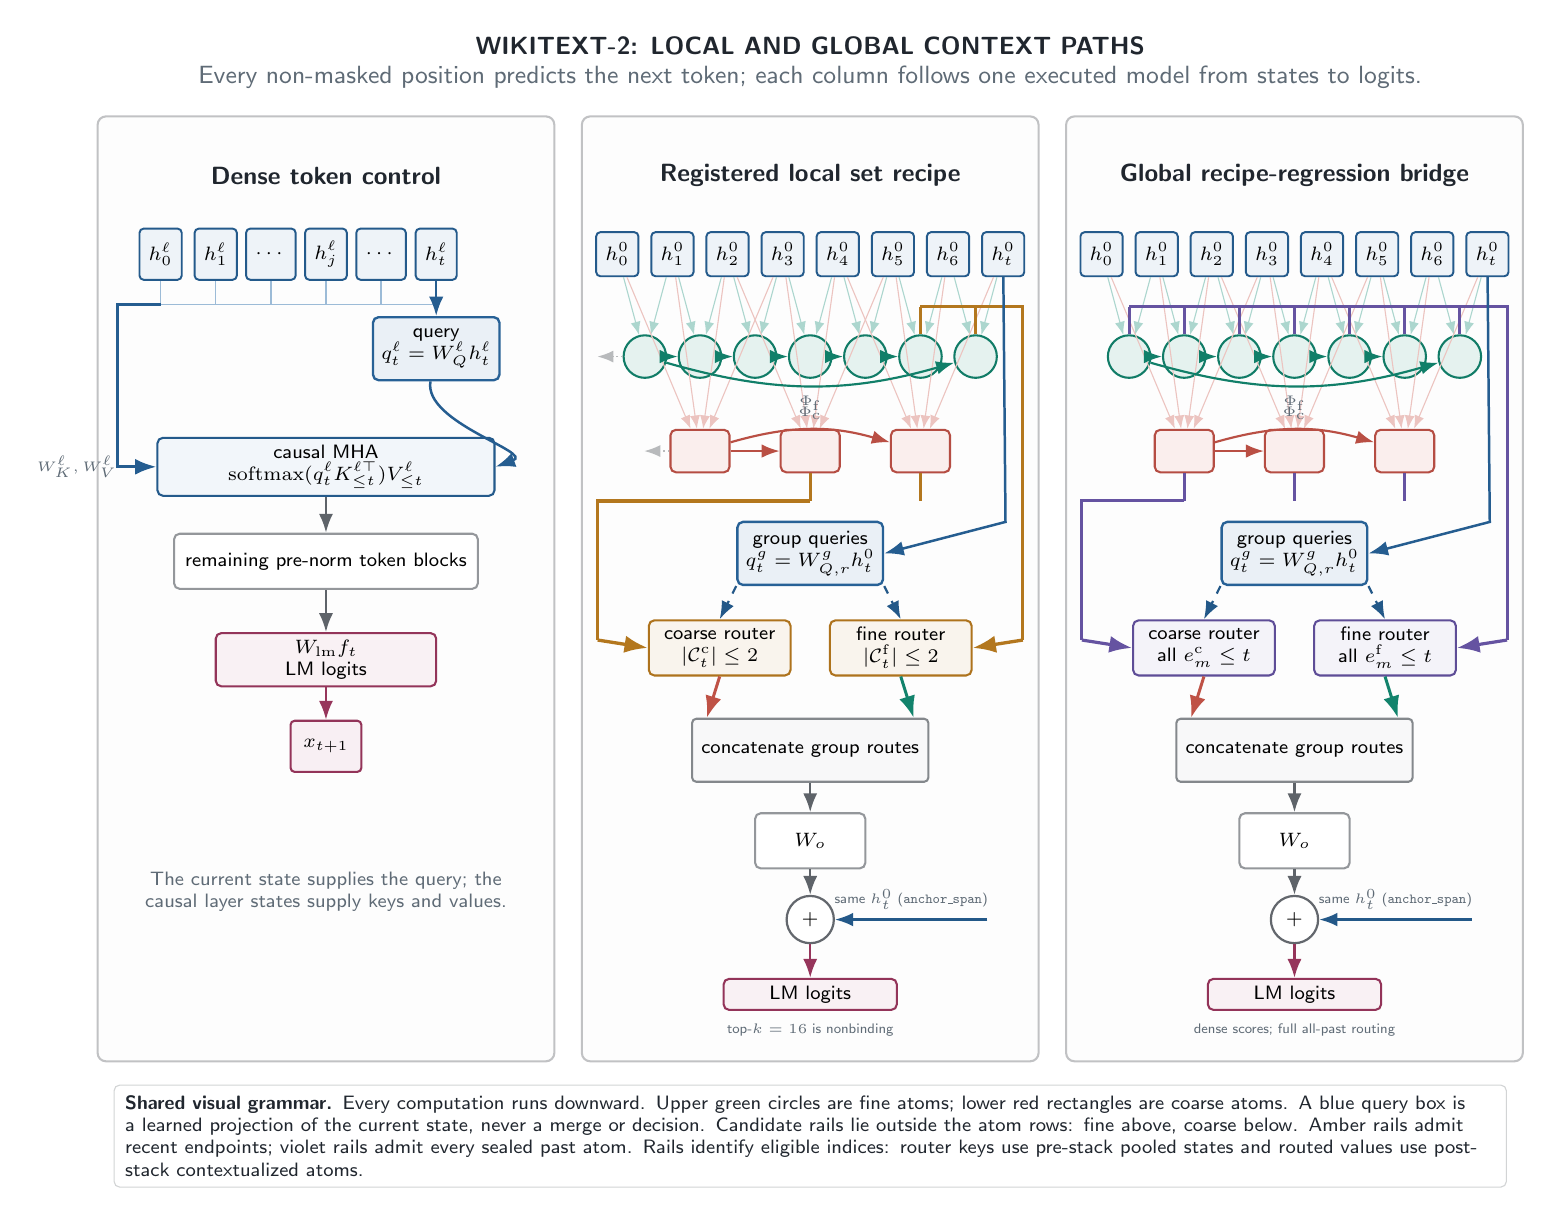
\begin{tikzpicture}[x=1cm,y=1cm]
\node[title] at (0,9.20) {WIKITEXT-2: LOCAL AND GLOBAL CONTEXT PATHS};
\node[subtitle] at (0,8.80)
  {Every non-masked position predicts the next token; each column follows one executed model from states to logits.};

\foreach \cx/\name in {-6.15/tok,0/loc,6.15/glo}
  \node[panel, minimum width=58mm, minimum height=120mm] (\name panel) at (\cx,2.30) {};
\node[paneltitle] at (-6.15,7.55) {Dense token control};
\node[paneltitle] at (0,7.55) {Registered local set recipe};
\node[paneltitle] at (6.15,7.55) {Global recipe-regression bridge};

% Token column: current state makes Q; the causal prefix makes K,V.
\foreach \x/\name/\lab in {-8.25/t0/$h_0^\ell$,-7.55/t1/$h_1^\ell$,-6.85/t2/$\cdots$,-6.15/t3/$h_j^\ell$,-5.45/t4/$\cdots$,-4.75/tt/$h_t^\ell$}
  \node[token, minimum width=5.2mm] (\name) at (\x,6.55) {\lab};
\foreach \name in {t0,t1,t2,t3,t4,tt} \draw[kvtap] (\name.south)--++(0,-0.30);
\draw[kvtap] ($(t0.south)+(0,-0.30)$)--($(tt.south)+(0,-0.30)$);
\node[query] (tq) at (-4.75,5.35) {query\\$q_t^\ell=W_Q^\ell h_t^\ell$};
\draw[tokenedge] (tt)--(tq);
\node[tokenmodule, text width=40mm] (tmha) at (-6.15,3.85)
  {causal MHA\\$\operatorname{softmax}(q_t^\ell K_{\le t}^{\ell\top})V_{\le t}^\ell$};
\draw[kvbus] ($(t0.south)+(0,-0.30)$)--++(-0.55,0) |- (tmha.west)
  node[pos=0.63,left,tiny] {$W_K^\ell,W_V^\ell$};
\draw[tokenedge] (tq) to[out=-100,in=20] (tmha.east);
\node[module, minimum width=28mm] (tblock) at (-6.15,2.65) {remaining pre-norm token blocks};
\node[loss, minimum width=28mm] (tlogits) at (-6.15,1.40) {$W_{\rm lm}f_t$\\LM logits};
\node[target] (tnext) at (-6.15,0.30) {$x_{t+1}$};
\draw[mergeedge] (tmha)--(tblock); \draw[mergeedge] (tblock)--(tlogits); \draw[lossedge] (tlogits)--(tnext);
\node[label, text width=48mm] at (-6.15,-1.55)
  {The current state supplies the query; the causal layer states supply keys and values.};

% Local set column: fixed upper/lower candidate lanes and vertical readout.
\foreach \x/\name/\lab in {-2.45/lx0/$h_0^0$,-1.75/lx1/$h_1^0$,-1.05/lx2/$h_2^0$,-0.35/lx3/$h_3^0$,0.35/lx4/$h_4^0$,1.05/lx5/$h_5^0$,1.75/lx6/$h_6^0$,2.45/lxt/$h_t^0$}
  \node[token, minimum width=4.8mm, minimum height=5.6mm] (\name) at (\x,6.55) {\lab};
\foreach \x/\name in {-2.10/lf0,-1.40/lf1,-0.70/lf2,0/lf3,0.70/lf4,1.40/lf5,2.10/lf6}
  \node[fineatom] (\name) at (\x,5.25) {};
\foreach \x/\name in {-1.40/lc0,0/lc1,1.40/lc2}
  \node[coarseatom] (\name) at (\x,4.05) {};
\foreach \a/\b/\f in {lx0/lx1/lf0,lx1/lx2/lf1,lx2/lx3/lf2,lx3/lx4/lf3,lx4/lx5/lf4,lx5/lx6/lf5,lx6/lxt/lf6}
  {\draw[poolfine] (\a)--(\f); \draw[poolfine] (\b)--(\f);}
\foreach \a/\b/\c/\d/\s in {lx0/lx1/lx2/lx3/lc0,lx2/lx3/lx4/lx5/lc1,lx4/lx5/lx6/lxt/lc2}
  {\draw[poolcoarse] (\a)--(\s); \draw[poolcoarse] (\b)--(\s); \draw[poolcoarse] (\c)--(\s); \draw[poolcoarse] (\d)--(\s);}
\foreach \a/\b in {lf0/lf1,lf1/lf2,lf2/lf3,lf3/lf4,lf4/lf5} \draw[causalFine] (\a)--(\b);
\draw[causalCoarse] (lc0)--(lc1);
\draw[causalFine] (lf0) to[bend right=16] node[below,tiny] {$\Phi_{\rm f}$} (lf6);
\draw[causalCoarse] (lc0) to[bend left=16] node[above,tiny] {$\Phi_{\rm c}$} (lc2);
% Fine candidates always use the lane above the fine row.
\coordinate (lfbus) at ($(lf5.north)+(0,0.35)$);
\foreach \a in {lf5,lf6} \draw[localbus] (\a.north)--(\a.north |- lfbus);
\draw[localbus] (lfbus)-|(2.70,1.65);
% Coarse candidates always use the lane below the coarse row.
\coordinate (lcbus) at ($(lc1.south)+(0,-0.35)$);
\foreach \a in {lc1,lc2} \draw[localbus] (\a.south)--(\a.south |- lcbus);
\draw[localbus] (lcbus)-|(-2.70,1.65);
\draw[excluded] (lf0.west)--++(-0.32,0); \draw[excluded] (lc0.west)--++(-0.32,0);
\node[query] (lq) at (0,2.75) {group queries\\$q_t^g=W_{Q,r}^g h_t^0$};
\draw[tokenedge] (lxt) -- (2.48,3.15) -- (lq.east);
\node[localmodule, minimum width=18mm] (lcr) at (-1.15,1.55) {coarse router\\$|\mathcal C_t^{\rm c}|\le2$};
\node[localmodule, minimum width=18mm] (lfr) at (1.15,1.55) {fine router\\$|\mathcal C_t^{\rm f}|\le2$};
\draw[localroute] (-2.70,1.65)--(lcr.west); \draw[localroute] (2.70,1.65)--(lfr.east);
\draw[queryedge] (lq.south west)--(lcr.north); \draw[queryedge] (lq.south east)--(lfr.north);
\node[merge] (lmerge) at (0,0.25) {concatenate group routes};
\draw[coarseout] (lcr.south)--($(lmerge.north west)+(0.20,0)$);
\draw[fineout] (lfr.south)--($(lmerge.north east)+(-0.20,0)$);
\node[module, minimum width=14mm] (lwo) at (0,-0.90) {$W_o$};
\node[addnode] (ladd) at (0,-1.90) {$+$};
\node[loss, minimum width=22mm] (llogits) at (0,-2.85) {LM logits};
\draw[mergeedge] (lmerge)--(lwo); \draw[mergeedge] (lwo)--(ladd); \draw[lossedge] (ladd)--(llogits);
\draw[anchorinput] (2.25,-1.90)--(ladd.east) node[midway,above,tiny] {same $h_t^0$ (\texttt{anchor\_span})};
\node[tiny] at (0,-3.30) {top-$k=16$ is nonbinding};

% Global set column, using exactly the same geometry as the local column.
\foreach \x/\name/\lab in {3.70/gx0/$h_0^0$,4.40/gx1/$h_1^0$,5.10/gx2/$h_2^0$,5.80/gx3/$h_3^0$,6.50/gx4/$h_4^0$,7.20/gx5/$h_5^0$,7.90/gx6/$h_6^0$,8.60/gxt/$h_t^0$}
  \node[token, minimum width=4.8mm, minimum height=5.6mm] (\name) at (\x,6.55) {\lab};
\foreach \x/\name in {4.05/gf0,4.75/gf1,5.45/gf2,6.15/gf3,6.85/gf4,7.55/gf5,8.25/gf6}
  \node[fineatom] (\name) at (\x,5.25) {};
\foreach \x/\name in {4.75/gc0,6.15/gc1,7.55/gc2}
  \node[coarseatom] (\name) at (\x,4.05) {};
\foreach \a/\b/\f in {gx0/gx1/gf0,gx1/gx2/gf1,gx2/gx3/gf2,gx3/gx4/gf3,gx4/gx5/gf4,gx5/gx6/gf5,gx6/gxt/gf6}
  {\draw[poolfine] (\a)--(\f); \draw[poolfine] (\b)--(\f);}
\foreach \a/\b/\c/\d/\s in {gx0/gx1/gx2/gx3/gc0,gx2/gx3/gx4/gx5/gc1,gx4/gx5/gx6/gxt/gc2}
  {\draw[poolcoarse] (\a)--(\s); \draw[poolcoarse] (\b)--(\s); \draw[poolcoarse] (\c)--(\s); \draw[poolcoarse] (\d)--(\s);}
\foreach \a/\b in {gf0/gf1,gf1/gf2,gf2/gf3,gf3/gf4,gf4/gf5} \draw[causalFine] (\a)--(\b);
\draw[causalCoarse] (gc0)--(gc1);
\draw[causalFine] (gf0) to[bend right=16] node[below,tiny] {$\Phi_{\rm f}$} (gf6);
\draw[causalCoarse] (gc0) to[bend left=16] node[above,tiny] {$\Phi_{\rm c}$} (gc2);
\coordinate (gfbus) at ($(gf0.north)+(0,0.35)$);
\foreach \a in {gf0,gf1,gf2,gf3,gf4,gf5,gf6} \draw[globalbus] (\a.north)--(\a.north |- gfbus);
\draw[globalbus] (gfbus)-|(8.85,1.65);
\coordinate (gcbus) at ($(gc0.south)+(0,-0.35)$);
\foreach \a in {gc0,gc1,gc2} \draw[globalbus] (\a.south)--(\a.south |- gcbus);
\draw[globalbus] (gcbus)-|(3.45,1.65);
\node[query] (gq) at (6.15,2.75) {group queries\\$q_t^g=W_{Q,r}^g h_t^0$};
\draw[tokenedge] (gxt) -- (8.63,3.15) -- (gq.east);
\node[globalmodule, minimum width=18mm] (gcr) at (5.00,1.55) {coarse router\\all $e_m^{\rm c}\le t$};
\node[globalmodule, minimum width=18mm] (gfr) at (7.30,1.55) {fine router\\all $e_m^{\rm f}\le t$};
\draw[globalroute] (3.45,1.65)--(gcr.west); \draw[globalroute] (8.85,1.65)--(gfr.east);
\draw[queryedge] (gq.south west)--(gcr.north); \draw[queryedge] (gq.south east)--(gfr.north);
\node[merge] (gmerge) at (6.15,0.25) {concatenate group routes};
\draw[coarseout] (gcr.south)--($(gmerge.north west)+(0.20,0)$);
\draw[fineout] (gfr.south)--($(gmerge.north east)+(-0.20,0)$);
\node[module, minimum width=14mm] (gwo) at (6.15,-0.90) {$W_o$};
\node[addnode] (gadd) at (6.15,-1.90) {$+$};
\node[loss, minimum width=22mm] (glogits) at (6.15,-2.85) {LM logits};
\draw[mergeedge] (gmerge)--(gwo); \draw[mergeedge] (gwo)--(gadd); \draw[lossedge] (gadd)--(glogits);
\draw[anchorinput] (8.40,-1.90)--(gadd.east) node[midway,above,tiny] {same $h_t^0$ (\texttt{anchor\_span})};
\node[tiny] at (6.15,-3.30) {dense scores; full all-past routing};

\node[note, text width=174mm] at (0,-4.65)
  {\textbf{Shared visual grammar.} Every computation runs downward.  Upper green circles are fine atoms; lower red rectangles are coarse atoms.  A blue query box is a learned projection of the current state, never a merge or decision.  Candidate rails lie outside the atom rows: fine above, coarse below.  Amber rails admit recent endpoints; violet rails admit every sealed past atom.  Rails identify eligible indices: router keys use pre-stack pooled states and routed values use post-stack contextualized atoms.};
\end{tikzpicture}

% ==========================================================================
% Page 2: MQAR. The same vertical grammar is used in both model columns.
% ==========================================================================
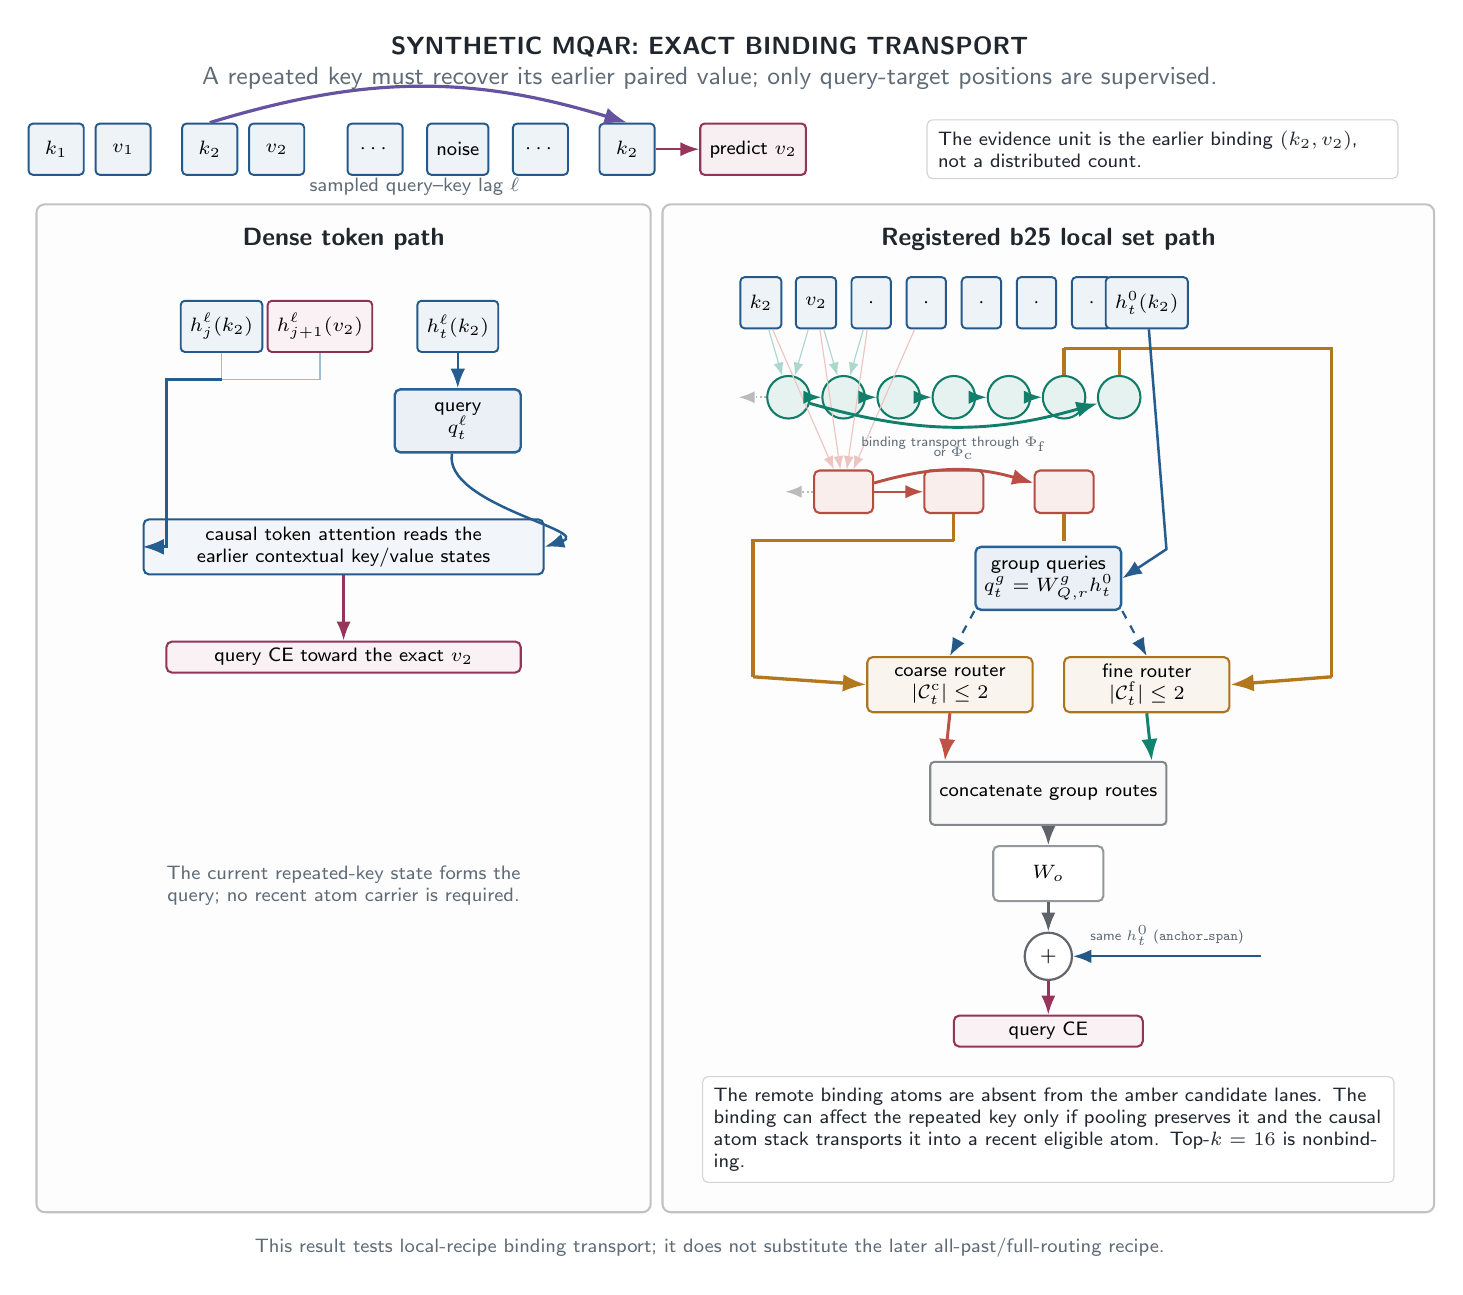
\begin{tikzpicture}[x=1cm,y=1cm]
\node[title] at (0,9.20) {SYNTHETIC MQAR: EXACT BINDING TRANSPORT};
\node[subtitle] at (0,8.80) {A repeated key must recover its earlier paired value; only query-target positions are supervised.};
\foreach \x/\name/\lab in {-8.3/mk1/$k_1$,-7.45/mv1/$v_1$,-6.35/mk2/$k_2$,-5.50/mv2/$v_2$,-4.25/mn0/$\cdots$,-3.20/mn1/noise,-2.15/mn2/$\cdots$,-1.05/mq2/$k_2$}
  \node[token] (\name) at (\x,7.90) {\lab};
\node[target] (mqt) at (0.55,7.90) {predict $v_2$};
\draw[lossedge] (mq2)--(mqt);
\draw[globalroute] (mk2.north) to[bend left=17] (mq2.north);
\node[label] at (-3.75,7.42) {sampled query--key lag $\ell$};
\node[note, text width=57mm] at (5.75,7.90)
  {The evidence unit is the earlier binding $(k_2,v_2)$, not a distributed count.};

\node[panel, minimum width=78mm, minimum height=128mm] at (-4.65,0.80) {};
\node[panel, minimum width=98mm, minimum height=128mm] at (4.30,0.80) {};
\node[paneltitle] at (-4.65,6.75) {Dense token path};
\node[paneltitle] at (4.30,6.75) {Registered b25 local set path};

% MQAR token path.
\node[token] (mtk) at (-6.20,5.65) {$h_j^\ell(k_2)$};
\node[token, draw=supervise!85!black, fill=supervise!7] (mtv) at (-4.95,5.65) {$h_{j+1}^\ell(v_2)$};
\node[token] (mtcur) at (-3.20,5.65) {$h_t^\ell(k_2)$};
\draw[kvtap] (mtk.south)--++(0,-0.34); \draw[kvtap] (mtv.south)--++(0,-0.34);
\draw[kvtap] ($(mtk.south)+(0,-0.34)$)--($(mtv.south)+(0,-0.34)$);
\node[query] (mtq) at (-3.20,4.45) {query\\$q_t^\ell$};
\draw[tokenedge] (mtcur)--(mtq);
\node[tokenmodule, text width=48mm] (mtmha) at (-4.65,2.85)
  {causal token attention reads the earlier contextual key/value states};
\draw[kvbus] ($(mtk.south)+(0,-0.34)$)--++(-0.70,0) |- (mtmha.west);
\draw[tokenedge] (mtq) to[out=-100,in=18] (mtmha.east);
\node[loss, minimum width=45mm] (mtloss) at (-4.65,1.45) {query CE toward the exact $v_2$};
\draw[lossedge] (mtmha)--(mtloss);
\node[label, text width=58mm] at (-4.65,-1.45)
  {The current repeated-key state forms the query; no recent atom carrier is required.};

% MQAR set path: banks and readout use the same lanes as every other set panel.
\foreach \x/\name/\lab in {0.65/ms0/$k_2$,1.35/ms1/$v_2$,2.05/ms2/$\cdot$,2.75/ms3/$\cdot$,3.45/ms4/$\cdot$,4.15/ms5/$\cdot$,4.85/ms6/$\cdot$,5.55/mst/$h_t^0(k_2)$}
  \node[token, minimum width=5mm] (\name) at (\x,5.95) {\lab};
\foreach \x/\name in {1.00/mf0,1.70/mf1,2.40/mf2,3.10/mf3,3.80/mf4,4.50/mf5,5.20/mf6}
  \node[fineatom] (\name) at (\x,4.75) {};
\foreach \x/\name in {1.70/mc0,3.10/mc1,4.50/mc2}
  \node[coarseatom] (\name) at (\x,3.55) {};
\draw[poolfine] (ms0)--(mf0); \draw[poolfine] (ms1)--(mf0);
\draw[poolfine] (ms1)--(mf1); \draw[poolfine] (ms2)--(mf1);
\foreach \a in {ms0,ms1,ms2,ms3} \draw[poolcoarse] (\a)--(mc0);
\foreach \a/\b in {mf0/mf1,mf1/mf2,mf2/mf3,mf3/mf4,mf4/mf5} \draw[causalFine] (\a)--(\b);
\draw[causalCoarse] (mc0)--(mc1);
\draw[causalFine, line width=1.05pt] (mf0) to[bend right=16] node[below,tiny] {binding transport through $\Phi_{\rm f}$} (mf6);
\draw[causalCoarse, line width=1.05pt] (mc0) to[bend left=16] node[above,tiny] {or $\Phi_{\rm c}$} (mc2);
\coordinate (mfbus) at ($(mf5.north)+(0,0.34)$);
\foreach \a in {mf5,mf6} \draw[localbus] (\a.north)--(\a.north |- mfbus);
\draw[localbus] (mfbus)-|(7.90,1.20);
\coordinate (mcbus) at ($(mc1.south)+(0,-0.34)$);
\foreach \a in {mc1,mc2} \draw[localbus] (\a.south)--(\a.south |- mcbus);
\draw[localbus] (mcbus)-|(0.55,1.20);
\draw[excluded] (mf0.west)--++(-0.35,0); \draw[excluded] (mc0.west)--++(-0.35,0);
\node[query] (msq) at (4.30,2.45) {group queries\\$q_t^g=W_{Q,r}^g h_t^0$};
\draw[tokenedge] (mst) -- (5.80,2.82) -- (msq.east);
\node[localmodule, minimum width=21mm] (mscr) at (3.05,1.10) {coarse router\\$|\mathcal C_t^{\rm c}|\le2$};
\node[localmodule, minimum width=21mm] (msfr) at (5.55,1.10) {fine router\\$|\mathcal C_t^{\rm f}|\le2$};
\draw[localroute] (0.55,1.20)--(mscr.west); \draw[localroute] (7.90,1.20)--(msfr.east);
\draw[queryedge] (msq.south west)--(mscr.north); \draw[queryedge] (msq.south east)--(msfr.north);
\node[merge] (msmerge) at (4.30,-0.28) {concatenate group routes};
\draw[coarseout] (mscr.south)--($(msmerge.north west)+(0.20,0)$);
\draw[fineout] (msfr.south)--($(msmerge.north east)+(-0.20,0)$);
\node[module, minimum width=14mm] (mswo) at (4.30,-1.30) {$W_o$};
\node[addnode] (msadd) at (4.30,-2.35) {$+$};
\node[loss, minimum width=24mm] (msloss) at (4.30,-3.30) {query CE};
\draw[mergeedge] (msmerge)--(mswo); \draw[mergeedge] (mswo)--(msadd); \draw[lossedge] (msadd)--(msloss);
\draw[anchorinput] (7.00,-2.35)--(msadd.east) node[midway,above,tiny] {same $h_t^0$ (\texttt{anchor\_span})};
\node[note, text width=85mm] at (4.30,-4.55)
  {The remote binding atoms are absent from the amber candidate lanes.  The binding can affect the repeated key only if pooling preserves it and the causal atom stack transports it into a recent eligible atom.  Top-$k=16$ is nonbinding.};
\node[label, text width=170mm] at (0,-6.05)
  {This result tests local-recipe binding transport; it does not substitute the later all-past/full-routing recipe.};
\end{tikzpicture}

% ==========================================================================
% Page 3: natural repeated-bigram AR, three vertical model columns.
% ==========================================================================
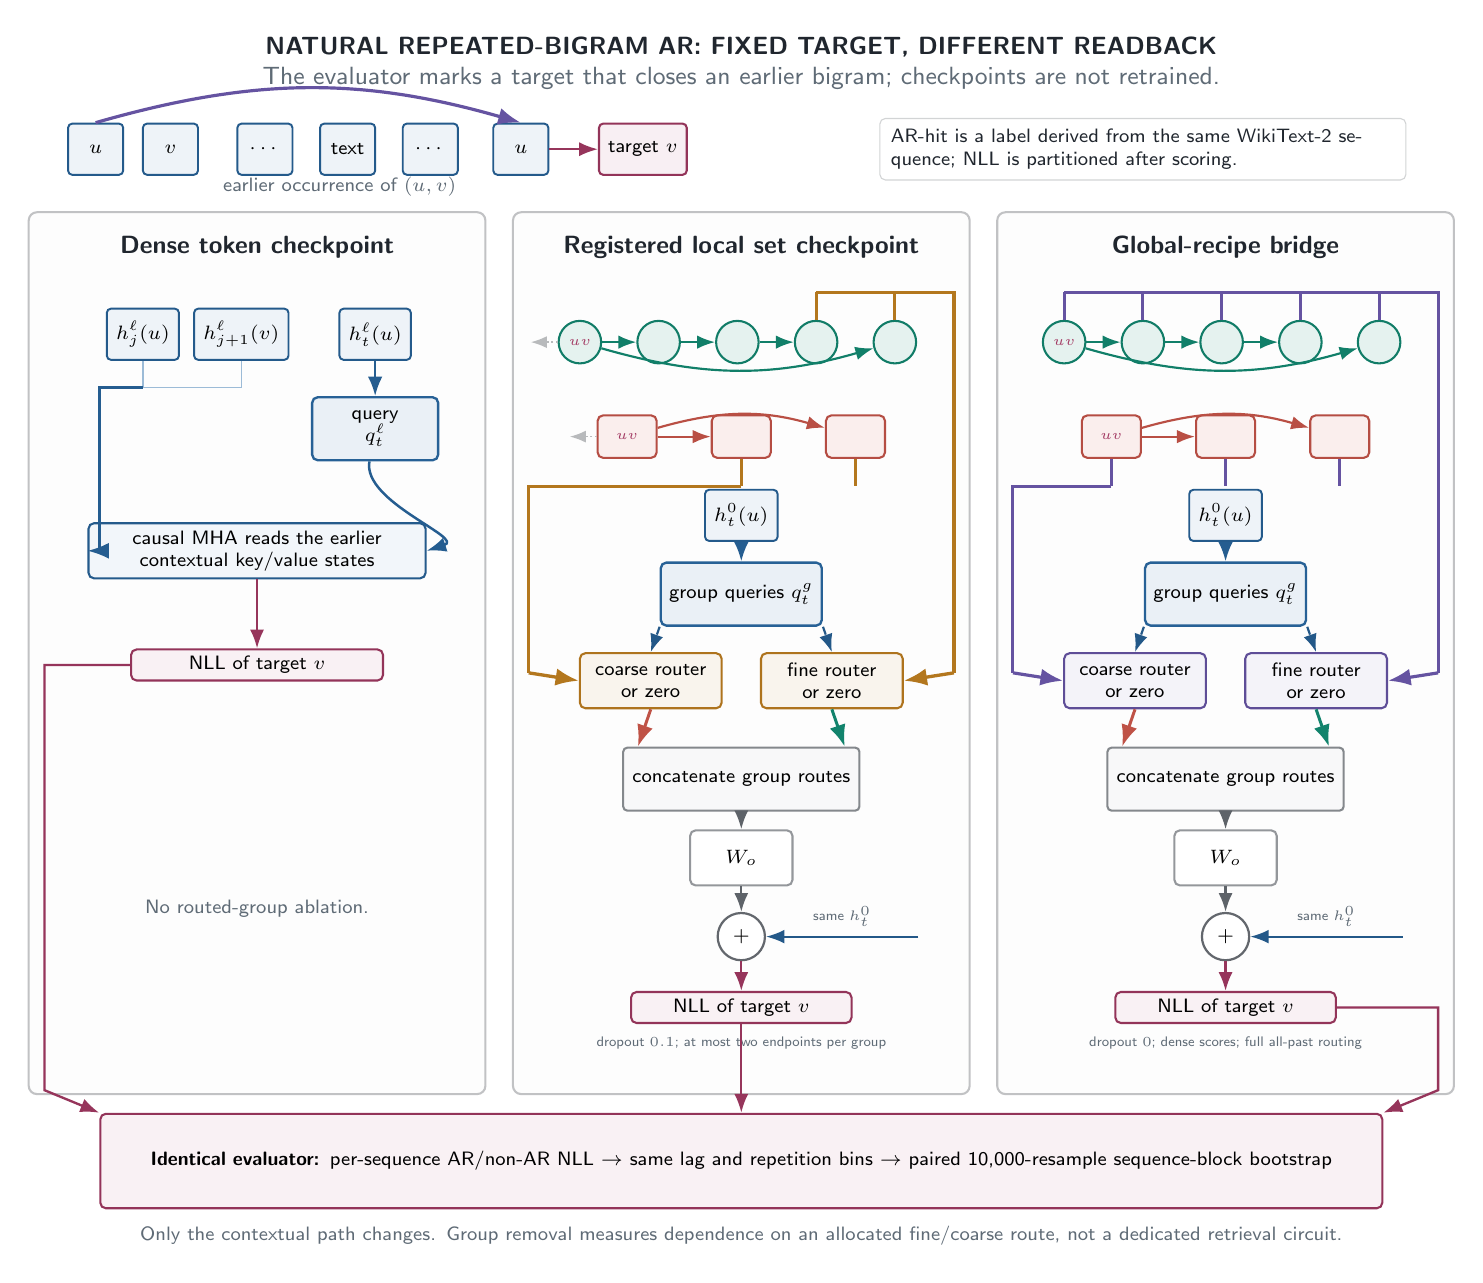
\begin{tikzpicture}[x=1cm,y=1cm]
\node[title] at (0,9.20) {NATURAL REPEATED-BIGRAM AR: FIXED TARGET, DIFFERENT READBACK};
\node[subtitle] at (0,8.80) {The evaluator marks a target that closes an earlier bigram; checkpoints are not retrained.};
\foreach \x/\name/\lab in {-8.2/aru1/$u$,-7.25/arv1/$v$,-6.05/ar0/$\cdots$,-5.00/ar1/text,-3.95/ar2/$\cdots$,-2.80/aru2/$u$}
  \node[token] (\name) at (\x,7.90) {\lab};
\node[target] (arv2) at (-1.25,7.90) {target $v$};
\draw[lossedge] (aru2)--(arv2); \draw[globalroute] (aru1.north) to[bend left=16] (aru2.north);
\node[label] at (-5.10,7.42) {earlier occurrence of $(u,v)$};
\node[note, text width=64mm] at (5.10,7.90)
  {AR-hit is a label derived from the same WikiText-2 sequence; NLL is partitioned after scoring.};

\foreach \cx/\name in {-6.15/art,0/arl,6.15/arg}
  \node[panel, minimum width=58mm, minimum height=112mm] (\name panel) at (\cx,1.50) {};
\node[paneltitle] at (-6.15,6.65) {Dense token checkpoint};
\node[paneltitle] at (0,6.65) {Registered local set checkpoint};
\node[paneltitle] at (6.15,6.65) {Global-recipe bridge};

% AR token column.
\node[token] (art0) at (-7.60,5.55) {$h_j^\ell(u)$};
\node[token] (art1) at (-6.35,5.55) {$h_{j+1}^\ell(v)$};
\node[token] (artt) at (-4.65,5.55) {$h_t^\ell(u)$};
\draw[kvtap] (art0.south)--++(0,-0.34); \draw[kvtap] (art1.south)--++(0,-0.34);
\draw[kvtap] ($(art0.south)+(0,-0.34)$)--($(art1.south)+(0,-0.34)$);
\node[query] (artq) at (-4.65,4.35) {query\\$q_t^\ell$};
\draw[tokenedge] (artt)--(artq);
\node[tokenmodule, text width=40mm] (artmha) at (-6.15,2.80)
  {causal MHA reads the earlier contextual key/value states};
\draw[kvbus] ($(art0.south)+(0,-0.34)$)--++(-0.55,0) |- (artmha.west);
\draw[tokenedge] (artq) to[out=-100,in=18] (artmha.east);
\node[loss, minimum width=32mm] (artloss) at (-6.15,1.35) {NLL of target $v$};
\draw[lossedge] (artmha)--(artloss);
\node[label] at (-6.15,-1.75) {No routed-group ablation.};

% AR local set column.
\foreach \x/\name in {-2.05/arf0,-1.05/arf1,-0.05/arf2,0.95/arf3,1.95/arf4} \node[fineatom] (\name) at (\x,5.45) {};
\foreach \x/\name in {-1.45/arc0,0/arc1,1.45/arc2} \node[coarseatom] (\name) at (\x,4.25) {};
\node[font=\tiny,text=supervise] at (arf0.center) {$uv$}; \node[font=\tiny,text=supervise] at (arc0.center) {$uv$};
\foreach \a/\b in {arf0/arf1,arf1/arf2,arf2/arf3} \draw[causalFine] (\a)--(\b);
\draw[causalCoarse] (arc0)--(arc1);
\draw[causalFine] (arf0) to[bend right=16] (arf4); \draw[causalCoarse] (arc0) to[bend left=16] (arc2);
\coordinate (arfbus) at ($(arf3.north)+(0,0.35)$);
\foreach \a in {arf3,arf4} \draw[localbus] (\a.north)--(\a.north |- arfbus);
\draw[localbus] (arfbus)-|(2.70,1.25);
\coordinate (arcbus) at ($(arc1.south)+(0,-0.35)$);
\foreach \a in {arc1,arc2} \draw[localbus] (\a.south)--(\a.south |- arcbus);
\draw[localbus] (arcbus)-|(-2.70,1.25);
\draw[excluded] (arf0.west)--++(-0.34,0); \draw[excluded] (arc0.west)--++(-0.34,0);
\node[token] (arlt) at (0,3.25) {$h_t^0(u)$};
\node[query] (arlq) at (0,2.25) {group queries $q_t^g$}; \draw[tokenedge] (arlt)--(arlq);
\node[localmodule, minimum width=18mm] (arlcr) at (-1.15,1.15) {coarse router\\or zero};
\node[localmodule, minimum width=18mm] (arlfr) at (1.15,1.15) {fine router\\or zero};
\draw[localroute] (-2.70,1.25)--(arlcr.west); \draw[localroute] (2.70,1.25)--(arlfr.east);
\draw[queryedge] (arlq.south west)--(arlcr.north); \draw[queryedge] (arlq.south east)--(arlfr.north);
\node[merge] (arlmerge) at (0,-0.10) {concatenate group routes};
\draw[coarseout] (arlcr.south)--($(arlmerge.north west)+(0.20,0)$);
\draw[fineout] (arlfr.south)--($(arlmerge.north east)+(-0.20,0)$);
\node[module, minimum width=13mm] (arlwo) at (0,-1.10) {$W_o$};
\node[addnode] (arladd) at (0,-2.10) {$+$};
\node[loss, minimum width=28mm] (arlloss) at (0,-3.00) {NLL of target $v$};
\draw[mergeedge] (arlmerge)--(arlwo); \draw[mergeedge] (arlwo)--(arladd); \draw[lossedge] (arladd)--(arlloss);
\draw[anchorinput] (2.25,-2.10)--(arladd.east) node[midway,above,tiny] {same $h_t^0$};
\node[tiny] at (0,-3.45) {dropout $0.1$; at most two endpoints per group};

% AR global set column, identical geometry.
\foreach \x/\name in {4.10/argf0,5.10/argf1,6.10/argf2,7.10/argf3,8.10/argf4} \node[fineatom] (\name) at (\x,5.45) {};
\foreach \x/\name in {4.70/argc0,6.15/argc1,7.60/argc2} \node[coarseatom] (\name) at (\x,4.25) {};
\node[font=\tiny,text=supervise] at (argf0.center) {$uv$}; \node[font=\tiny,text=supervise] at (argc0.center) {$uv$};
\foreach \a/\b in {argf0/argf1,argf1/argf2,argf2/argf3} \draw[causalFine] (\a)--(\b);
\draw[causalCoarse] (argc0)--(argc1);
\draw[causalFine] (argf0) to[bend right=16] (argf4); \draw[causalCoarse] (argc0) to[bend left=16] (argc2);
\coordinate (argfbus) at ($(argf0.north)+(0,0.35)$);
\foreach \a in {argf0,argf1,argf2,argf3,argf4} \draw[globalbus] (\a.north)--(\a.north |- argfbus);
\draw[globalbus] (argfbus)-|(8.85,1.25);
\coordinate (argcbus) at ($(argc0.south)+(0,-0.35)$);
\foreach \a in {argc0,argc1,argc2} \draw[globalbus] (\a.south)--(\a.south |- argcbus);
\draw[globalbus] (argcbus)-|(3.45,1.25);
\node[token] (argt) at (6.15,3.25) {$h_t^0(u)$};
\node[query] (argq) at (6.15,2.25) {group queries $q_t^g$}; \draw[tokenedge] (argt)--(argq);
\node[globalmodule, minimum width=18mm] (argcr) at (5.00,1.15) {coarse router\\or zero};
\node[globalmodule, minimum width=18mm] (argfr) at (7.30,1.15) {fine router\\or zero};
\draw[globalroute] (3.45,1.25)--(argcr.west); \draw[globalroute] (8.85,1.25)--(argfr.east);
\draw[queryedge] (argq.south west)--(argcr.north); \draw[queryedge] (argq.south east)--(argfr.north);
\node[merge] (argmerge) at (6.15,-0.10) {concatenate group routes};
\draw[coarseout] (argcr.south)--($(argmerge.north west)+(0.20,0)$);
\draw[fineout] (argfr.south)--($(argmerge.north east)+(-0.20,0)$);
\node[module, minimum width=13mm] (argwo) at (6.15,-1.10) {$W_o$};
\node[addnode] (argadd) at (6.15,-2.10) {$+$};
\node[loss, minimum width=28mm] (argloss) at (6.15,-3.00) {NLL of target $v$};
\draw[mergeedge] (argmerge)--(argwo); \draw[mergeedge] (argwo)--(argadd); \draw[lossedge] (argadd)--(argloss);
\draw[anchorinput] (8.40,-2.10)--(argadd.east) node[midway,above,tiny] {same $h_t^0$};
\node[tiny] at (6.15,-3.45) {dropout $0$; dense scores; full all-past routing};

\node[loss, text width=160mm, minimum height=12mm] (areval) at (0,-4.95)
  {\textbf{Identical evaluator:} per-sequence AR/non-AR NLL $\rightarrow$ same lag and repetition bins $\rightarrow$ paired 10,000-resample sequence-block bootstrap};
\draw[lossedge] (artloss.west)--(-8.85,1.35)--(-8.85,-4.05)--(areval.north west);
\draw[lossedge] (arlloss)--(0,-4.05)--(areval.north);
\draw[lossedge] (argloss.east)--(8.85,-3.00)--(8.85,-4.05)--(areval.north east);
\node[label, text width=168mm] at (0,-5.90)
  {Only the contextual path changes.  Group removal measures dependence on an allocated fine/coarse route, not a dedicated retrieval circuit.};
\end{tikzpicture}

% ==========================================================================
% Page 4: LCA. The three model columns use the same vertical grammar.
% ==========================================================================
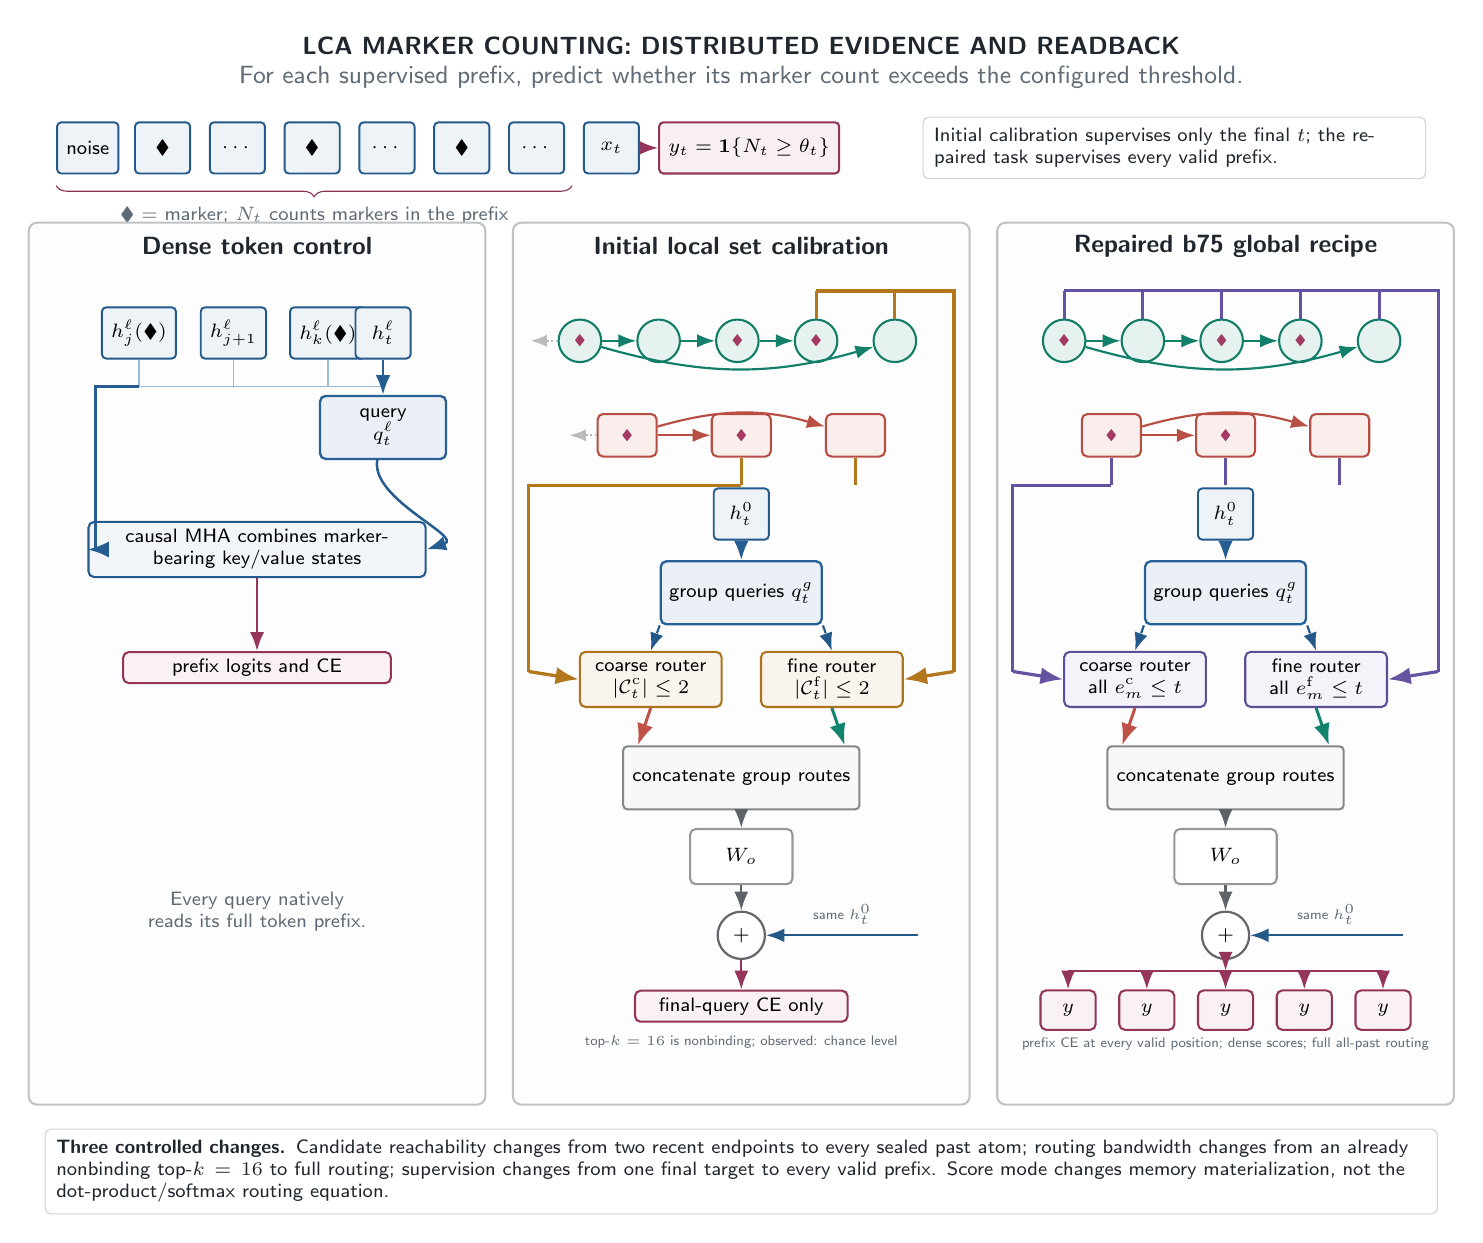
\begin{tikzpicture}[x=1cm,y=1cm]
\node[title] at (0,9.20) {LCA MARKER COUNTING: DISTRIBUTED EVIDENCE AND READBACK};
\node[subtitle] at (0,8.80) {For each supervised prefix, predict whether its marker count exceeds the configured threshold.};
\foreach \x/\name/\lab in {-8.3/lx0/noise,-7.35/lm0/$\blacklozenge$,-6.40/lx1/$\cdots$,-5.45/lm1/$\blacklozenge$,-4.50/lx2/$\cdots$,-3.55/lm2/$\blacklozenge$,-2.60/lx3/$\cdots$,-1.65/lxt/$x_t$}
  \node[token] (\name) at (\x,7.90) {\lab};
\node[target] (lyt) at (0.10,7.90) {$y_t=\mathbf1\{N_t\ge\theta_t\}$}; \draw[lossedge] (lxt)--(lyt);
\draw[decorate, decoration={brace,mirror,amplitude=4pt}, draw=supervise!85!black]
  (-8.70,7.42)--(-2.15,7.42) node[midway,below=4pt,label] {$\blacklozenge$ = marker; $N_t$ counts markers in the prefix};
\node[note, text width=61mm] at (5.50,7.90)
  {Initial calibration supervises only the final $t$; the repaired task supervises every valid prefix.};

\foreach \cx/\name in {-6.15/ltt,0/lll,6.15/lgg}
  \node[panel, minimum width=58mm, minimum height=112mm] (\name panel) at (\cx,1.35) {};
\node[paneltitle] at (-6.15,6.65) {Dense token control};
\node[paneltitle] at (0,6.65) {Initial local set calibration};
\node[paneltitle] at (6.15,6.65) {Repaired b75 global recipe};

% LCA token column.
\foreach \x/\name/\lab in {-7.65/lt0/$h_j^\ell(\blacklozenge)$,-6.45/lt1/$h_{j+1}^\ell$,-5.25/lt2/$h_k^\ell(\blacklozenge)$,-4.55/lttt/$h_t^\ell$}
  \node[token] (\name) at (\x,5.55) {\lab};
\foreach \name in {lt0,lt1,lt2,lttt} \draw[kvtap] (\name.south)--++(0,-0.34);
\draw[kvtap] ($(lt0.south)+(0,-0.34)$)--($(lttt.south)+(0,-0.34)$);
\node[query] (lttq) at (-4.55,4.35) {query\\$q_t^\ell$}; \draw[tokenedge] (lttt)--(lttq);
\node[tokenmodule, text width=40mm] (lttmha) at (-6.15,2.80)
  {causal MHA combines marker-bearing key/value states};
\draw[kvbus] ($(lt0.south)+(0,-0.34)$)--++(-0.55,0) |- (lttmha.west);
\draw[tokenedge] (lttq) to[out=-100,in=18] (lttmha.east);
\node[loss, minimum width=34mm] (lttloss) at (-6.15,1.30) {prefix logits and CE};
\draw[lossedge] (lttmha)--(lttloss);
\node[label, text width=48mm] at (-6.15,-1.80) {Every query natively reads its full token prefix.};

% LCA local set column.
\foreach \x/\name in {-2.05/llf0,-1.05/llf1,-0.05/llf2,0.95/llf3,1.95/llf4} \node[fineatom] (\name) at (\x,5.45) {};
\foreach \x/\name in {-1.45/llc0,0/llc1,1.45/llc2} \node[coarseatom] (\name) at (\x,4.25) {};
\foreach \a in {llf0,llf2,llf3,llc0,llc1} \node[font=\tiny,text=supervise] at (\a.center) {$\blacklozenge$};
\foreach \a/\b in {llf0/llf1,llf1/llf2,llf2/llf3} \draw[causalFine] (\a)--(\b);
\draw[causalCoarse] (llc0)--(llc1);
\draw[causalFine] (llf0) to[bend right=16] (llf4); \draw[causalCoarse] (llc0) to[bend left=16] (llc2);
\coordinate (llfbus) at ($(llf3.north)+(0,0.35)$);
\foreach \a in {llf3,llf4} \draw[localbus] (\a.north)--(\a.north |- llfbus);
\draw[localbus] (llfbus)-|(2.70,1.25);
\coordinate (llcbus) at ($(llc1.south)+(0,-0.35)$);
\foreach \a in {llc1,llc2} \draw[localbus] (\a.south)--(\a.south |- llcbus);
\draw[localbus] (llcbus)-|(-2.70,1.25);
\draw[excluded] (llf0.west)--++(-0.34,0); \draw[excluded] (llc0.west)--++(-0.34,0);
\node[token] (llh) at (0,3.25) {$h_t^0$};
\node[query] (llq) at (0,2.25) {group queries $q_t^g$}; \draw[tokenedge] (llh)--(llq);
\node[localmodule, minimum width=18mm] (llcr) at (-1.15,1.15) {coarse router\\$|\mathcal C_t^{\rm c}|\le2$};
\node[localmodule, minimum width=18mm] (llfr) at (1.15,1.15) {fine router\\$|\mathcal C_t^{\rm f}|\le2$};
\draw[localroute] (-2.70,1.25)--(llcr.west); \draw[localroute] (2.70,1.25)--(llfr.east);
\draw[queryedge] (llq.south west)--(llcr.north); \draw[queryedge] (llq.south east)--(llfr.north);
\node[merge] (llmerge) at (0,-0.10) {concatenate group routes};
\draw[coarseout] (llcr.south)--($(llmerge.north west)+(0.20,0)$);
\draw[fineout] (llfr.south)--($(llmerge.north east)+(-0.20,0)$);
\node[module, minimum width=13mm] (llwo) at (0,-1.10) {$W_o$};
\node[addnode] (lladd) at (0,-2.10) {$+$};
\node[loss, minimum width=27mm] (llloss) at (0,-3.00) {final-query CE only};
\draw[mergeedge] (llmerge)--(llwo); \draw[mergeedge] (llwo)--(lladd); \draw[lossedge] (lladd)--(llloss);
\draw[anchorinput] (2.25,-2.10)--(lladd.east) node[midway,above,tiny] {same $h_t^0$};
\node[tiny] at (0,-3.45) {top-$k=16$ is nonbinding; observed: chance level};

% LCA global set column, same geometry.
\foreach \x/\name in {4.10/lgf0,5.10/lgf1,6.10/lgf2,7.10/lgf3,8.10/lgf4} \node[fineatom] (\name) at (\x,5.45) {};
\foreach \x/\name in {4.70/lgc0,6.15/lgc1,7.60/lgc2} \node[coarseatom] (\name) at (\x,4.25) {};
\foreach \a in {lgf0,lgf2,lgf3,lgc0,lgc1} \node[font=\tiny,text=supervise] at (\a.center) {$\blacklozenge$};
\foreach \a/\b in {lgf0/lgf1,lgf1/lgf2,lgf2/lgf3} \draw[causalFine] (\a)--(\b);
\draw[causalCoarse] (lgc0)--(lgc1);
\draw[causalFine] (lgf0) to[bend right=16] (lgf4); \draw[causalCoarse] (lgc0) to[bend left=16] (lgc2);
\coordinate (lgfbus) at ($(lgf0.north)+(0,0.35)$);
\foreach \a in {lgf0,lgf1,lgf2,lgf3,lgf4} \draw[globalbus] (\a.north)--(\a.north |- lgfbus);
\draw[globalbus] (lgfbus)-|(8.85,1.25);
\coordinate (lgcbus) at ($(lgc0.south)+(0,-0.35)$);
\foreach \a in {lgc0,lgc1,lgc2} \draw[globalbus] (\a.south)--(\a.south |- lgcbus);
\draw[globalbus] (lgcbus)-|(3.45,1.25);
\node[token] (lgh) at (6.15,3.25) {$h_t^0$};
\node[query] (lgq) at (6.15,2.25) {group queries $q_t^g$}; \draw[tokenedge] (lgh)--(lgq);
\node[globalmodule, minimum width=18mm] (lgcr) at (5.00,1.15) {coarse router\\all $e_m^{\rm c}\le t$};
\node[globalmodule, minimum width=18mm] (lgfr) at (7.30,1.15) {fine router\\all $e_m^{\rm f}\le t$};
\draw[globalroute] (3.45,1.25)--(lgcr.west); \draw[globalroute] (8.85,1.25)--(lgfr.east);
\draw[queryedge] (lgq.south west)--(lgcr.north); \draw[queryedge] (lgq.south east)--(lgfr.north);
\node[merge] (lgmerge) at (6.15,-0.10) {concatenate group routes};
\draw[coarseout] (lgcr.south)--($(lgmerge.north west)+(0.20,0)$);
\draw[fineout] (lgfr.south)--($(lgmerge.north east)+(-0.20,0)$);
\node[module, minimum width=13mm] (lgwo) at (6.15,-1.10) {$W_o$};
\node[addnode] (lgadd) at (6.15,-2.10) {$+$};
\draw[mergeedge] (lgmerge)--(lgwo); \draw[mergeedge] (lgwo)--(lgadd);
\draw[anchorinput] (8.40,-2.10)--(lgadd.east) node[midway,above,tiny] {same $h_t^0$};
\draw[lossedge] (lgadd)--(6.15,-2.55);
\draw[supervisionbus] (4.15,-2.55)--(8.15,-2.55);
\foreach \x/\name in {4.15/lgy0,5.15/lgy1,6.15/lgy2,7.15/lgy3,8.15/lgy4}
  {\node[loss, minimum width=7mm, minimum height=5mm, inner sep=1pt] (\name) at (\x,-3.05) {$y$};
   \draw[lossedge] (\x,-2.55)--(\name.north);}
\node[tiny] at (6.15,-3.48) {prefix CE at every valid position; dense scores; full all-past routing};

\node[note, text width=174mm] at (0,-5.10)
  {\textbf{Three controlled changes.}  Candidate reachability changes from two recent endpoints to every sealed past atom; routing bandwidth changes from an already nonbinding top-$k=16$ to full routing; supervision changes from one final target to every valid prefix.  Score mode changes memory materialization, not the dot-product/softmax routing equation.};
\end{tikzpicture}

\end{document}
